\documentclass{standalone}
\usepackage{pgfplots}
\pgfplotsset{compat=1.17}
\begin{document}
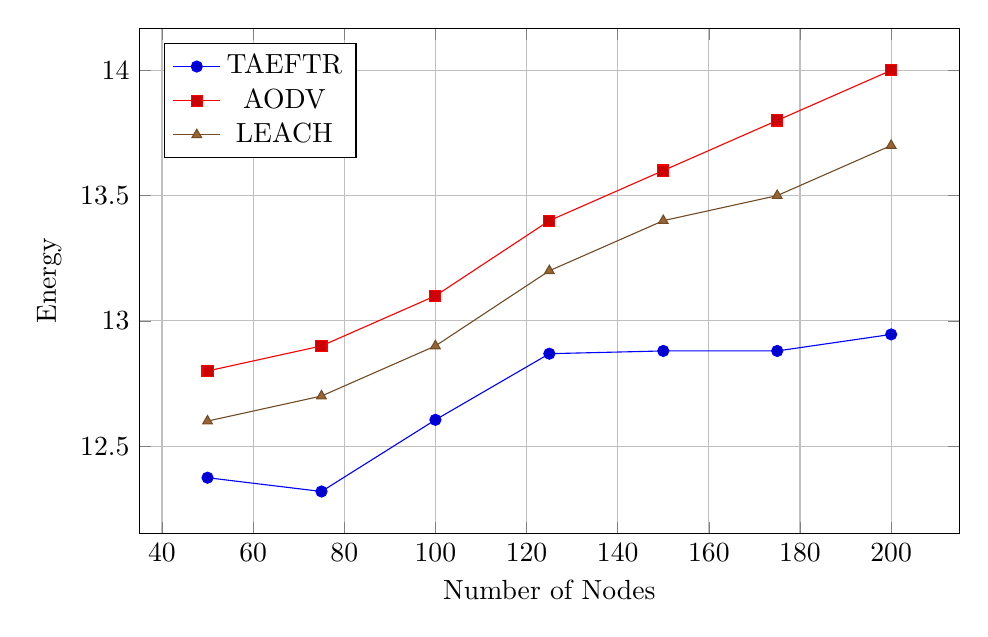
\begin{tikzpicture}
\begin{axis}[
width=12cm,height=8cm,
xlabel={Number of Nodes},
ylabel={Energy},
grid=major,
legend pos=north west]
\addplot+[mark=*] coordinates {(50,12.374)(75,12.319)(100,12.605)(125,12.869)(150,12.88)(175,12.88)(200,12.946)};
\addplot+[mark=square*] coordinates {(50,12.8)(75,12.9)(100,13.1)(125,13.4)(150,13.6)(175,13.8)(200,14)};
\addplot+[mark=triangle*] coordinates {(50,12.6)(75,12.7)(100,12.9)(125,13.2)(150,13.4)(175,13.5)(200,13.7)};
\legend{TAEFTR,AODV,LEACH}
\end{axis}
\end{tikzpicture}
\end{document}